Цифровое изображение естественно рассматривать как функцию на пиксельной сетке: $I: \{1, \dots, H\} \times \{1, \dots, W\} \to \mathbb{R}$, где значение $I(p)$ интерпретируется как яркость (для одноканальных изображений) или один из каналов цвета. Чтобы применить к нему аппарат персистентных гомологий, нужно (а) задать симплициальный комплекс $K$, отражающий геометрию решётки, и (б) определить на нём фильтрацию, согласованную с содержимым изображения. В качестве $K$ обычно берут кубический комплекс, в котором симплексами являются пиксели (нульмерные клетки), их рёбра (одномерные клетки), сцепляющие соседние пиксели, и квадраты (двумерные клетки), заполняющие промежутки между четвёрками соседей. Этот выбор естественен и хорошо поддерживается современными вычислительными библиотеками.

\paragraph{Подуровневая фильтрация по интенсивности.}
Простейшая фильтрация на изображении --- подуровневая по самой интенсивности. Положим $w(p) = I(p)$ и распространим $w$ на симплексы по правилу $w(\sigma) = \max_{p \in \sigma} w(p)$ (см.\ §\ref{ssec:basic-defs}). Семейство подкомплексов
\[
K_a = \{\sigma \in K : w(\sigma) \le a\}, \qquad a \in \mathbb{R},
\]
образует фильтрацию, отражающую <<рост>> области тёмных пикселей при увеличении порога $a$. Соответствующая диаграмма $\mathrm{Dgm}_0$ кодирует появление и исчезновение связных компонентов уровня, а $\mathrm{Dgm}_1$ --- появление и заполнение петель (одномерных дыр), что для изображения отпечатка пальца, к примеру, отвечает гребням и впадинам узора.

\paragraph{Направленные фильтрации и Persistent Homology Transform.}
Подуровневая фильтрация по интенсивности использует только значения функции и игнорирует пространственную ориентацию структур на изображении. Чтобы исправить это, в работе Turner, Mukherjee, Boyer (2014)~\cite{turnerPersistentHomologyTransform2014} было предложено рассматривать целое семейство направленных фильтраций, индексированных направлениями. Для каждого единичного вектора $v_\alpha = (\cos\alpha, \sin\alpha)$, $\alpha \in [0, 2\pi)$, определим функцию высоты
\[
w_\alpha(p) = \langle p, v_\alpha \rangle = p_x \cos\alpha + p_y \sin\alpha,
\]
и по ней построим подуровневую фильтрацию. Получающееся отображение
\[
\mathrm{PHT}: \alpha \mapsto \bigl( \mathrm{Dgm}_0(\alpha), \mathrm{Dgm}_1(\alpha) \bigr)
\]
называется \emph{Persistent Homology Transform} (PHT) и для кусочно-линейных поверхностей в $\mathbb{R}^2$/$\mathbb{R}^3$ является инъективным: знание диаграмм во всех направлениях позволяет восстановить форму объекта~\cite{turnerPersistentHomologyTransform2014}. Это делает PHT богатым по информации топологическим дескриптором формы, чувствительным к ориентации, в отличие от чисто радиально-симметричных характеристик.

На практике непрерывное семейство $\alpha \in [0, 2\pi)$ дискретизируется конечным набором направлений. В нашей реализации (см.\ \texttt{src/filtrations/pht.py}) по умолчанию используется $16$ равномерно распределённых углов $\alpha \in \{0^\circ, 22{.}5^\circ, \dots, 337{.}5^\circ\}$. Для каждого направления получается своя диаграмма с точками вида $(b, d)$; объединение всех таких диаграмм и составляет вход для модели. Чтобы модель могла различать диаграммы из разных направлений, к каждой точке прикрепляется метаинформация: гомологическая размерность, флаг типа фильтрации (sublevel/PHT), сам угол $\alpha$ и его синусоидальное позиционное кодирование. Таким образом, одна точка диаграммы превращается в небольшой вектор признаков, что естественным образом подаётся в нейронные сети, обрабатывающие неупорядоченные множества (см. §\ref{sec:embedding-task}).

\begin{figure}[ht]
\centering
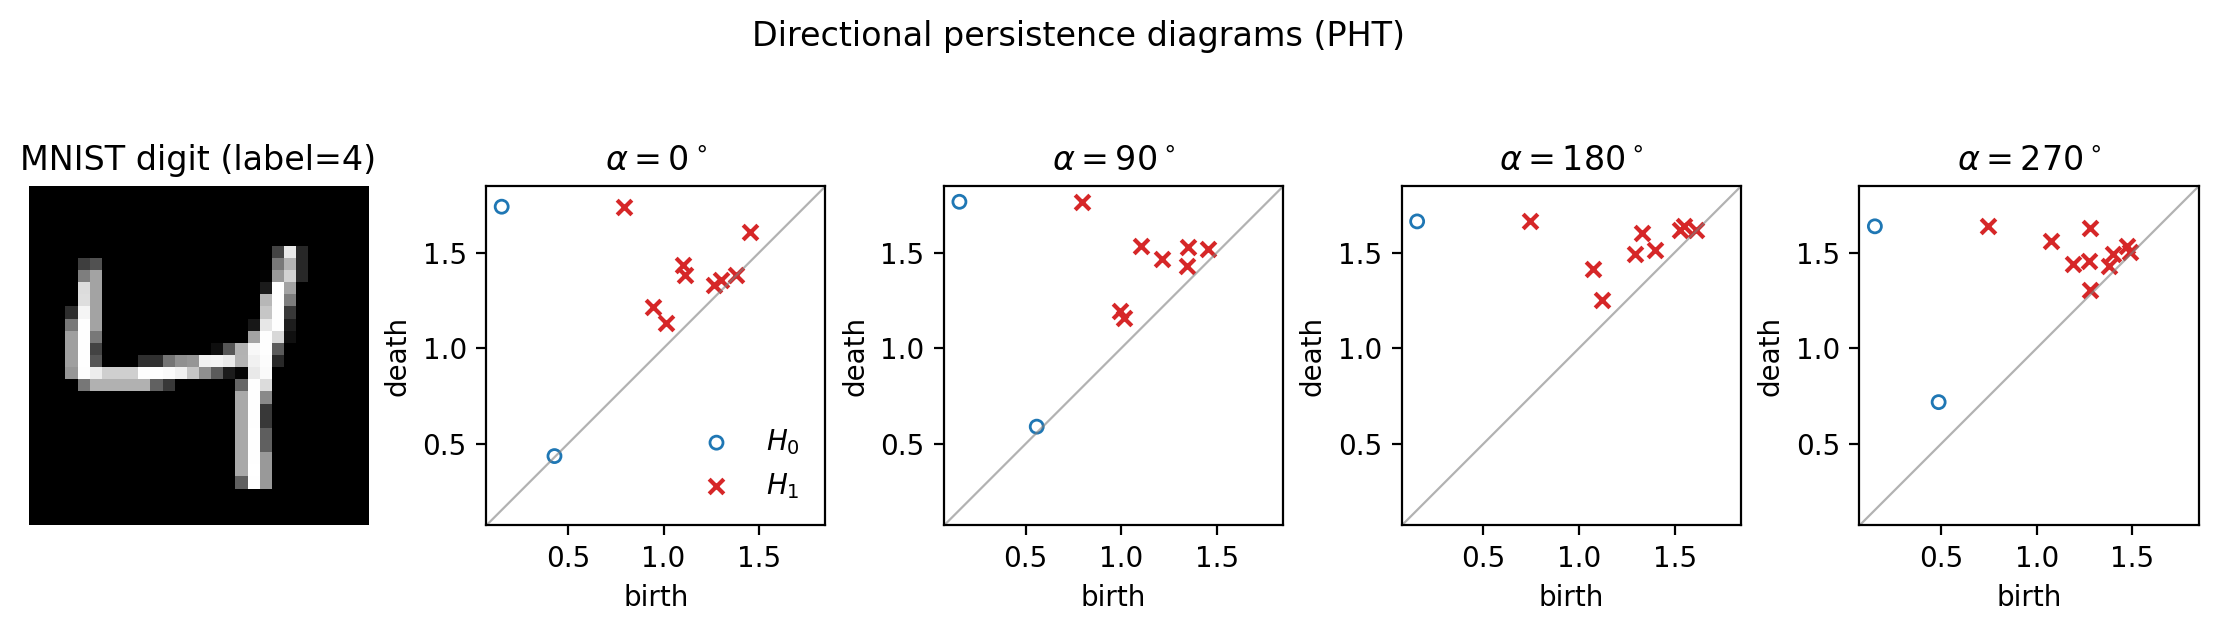
\includegraphics[width=\linewidth]{figures/mnist_directional_pht.png}
\caption{Пример изображения цифры из MNIST (слева) и соответствующие диаграммы персистентности, получаемые направленной фильтрацией для четырёх направлений $\alpha \in \{0^\circ, 90^\circ, 180^\circ, 270^\circ\}$ (справа). Точки $H_0$ и $H_1$ изображены разными маркерами; видно, как направление фильтрации перераспределяет точки между диаграммами и тем самым кодирует ориентацию структур на изображении.}
\label{fig:pht-illustration}
\end{figure}
